%\paragraph{}This chapter goes over 2 examples of tuning 2 distinct \ac{SLAM} algorithms(faster-lio and fast-livo2), using all three tuning algorithms implemented. Given that the purpose of this dissertation is to optimize \ac{SLAM} solutions, there is not much sense in comparing the effectiveness of faster-lio and fast-livo2. It was therefore decided that the focus of this section should instead be on showcasing the implemented tuning algorithms, according to a predefined tuning strategy.

\paragraph{}This chapter presents two case studies involving the tuning of two distinct \ac{SLAM} algorithms (Faster-LIO and Fast-LIVO2) using the three implemented tuning algorithms. Given that the primary objective of this dissertation is the optimization of \ac{SLAM} algorithms, a direct comparison of the performance of Faster-LIO and Fast-LIVO2 is not meaningful. Instead, the focus of this section is in showcasing how well the implemented tuning algorithms perform when compared with default parameters executions.

\section{Faster-LIO}

%\paragraph{}It is important, before tuning any hyperparameter, to run the algorithm with default parameters, to know what the \ac{RPE} is when no optimization is performed. Below is a table with the 5 run average of the \ac{APE} and \ac{RPE} for the faster-lio algorithm(table \ref{default-faster-lio}). These results were obtained with the parameter values specified in table \ref{default-faster-lio-params}.

\paragraph{}Prior to parameter tuning, Faster-LIO was evaluated using its default parameter configuration to establish a baseline for \ac{RPE}. Table \ref{default-faster-lio} presents the five-run average APE and RPE for Faster-LIO, obtained using the parameter values reported in Table \ref{default-faster-lio-params}.

\begin{table}[h]
\centering
\begin{tabular}{|l|l|}
\hline
APE (RMSE) & RPE (RMSE) \\ \hline
0.664834  & 0.015037  \\ \hline
\end{tabular}
\caption{Default parameter results (5 run average) for Faster-LIO}
\label{default-faster-lio}
\end{table}

\begin{table}[]
\centering
\begin{tabular}{|l|l|}
\hline
point\_filter\_num     & 3    \\ \hline
max\_iteration         & 3    \\ \hline
filter\_size\_map      & 0.5  \\ \hline
filter\_size\_surf     & 0.5  \\ \hline
cube\_side\_length     & 1000 \\ \hline
ivox\_grid\_resolution & 0.5  \\ \hline
esti\_plane\_threshold & 0.1  \\ \hline
\end{tabular}
\caption{Default parameter values for Faster-LIO}
\label{default-faster-lio-params}
\end{table}

\paragraph{}Before running Simulated Annealing, it is necessary to define the hyperparameters of the algorithm.

\paragraph{}Then, the following parameter space was devised. The two tables below present the parameter settings used for Simulated Annealing. The parameters are divided into two groups: discrete parameters (Table \ref{faster-lio-discrete-params-settings}) and continuous parameters (Table \ref{faster-lio-continuous-params-settings}).

%The below two tables show the configuration of the optimized faster-lio parameters for simulated annealing. They are separated into two tables: one for discrete parameters and one for continuous parameters.

\begin{table}[h]
\centering
\begin{tabular}{|c|c|c|c|c|}
\hline
Parameter          & Initial Value & Lower Bound & Upper Bound & delta max \\ \hline
point\_filter\_num & 20            & 2           & 50          & 8         \\ \hline
max\_iteration     & 10            & 3           & 50          & 5         \\ \hline
cube\_side\_length & 1100          & 700         & 2000        & 300       \\ \hline
\end{tabular}
\caption{Faster-LIO discrete parameter settings.}
\label{faster-lio-discrete-params-settings}
\end{table}

\begin{table}[h]
\centering
\begin{tabular}{|c|c|c|c|c|c|}
\hline
Parameter              & Initial Value & Lower Bound & Upper Bound & $\mu$     & $\sigma$     \\ \hline
filter\_size\_map      & 0.5           & 0.1         & 0.75        & -0.01 & 0.003 \\ \hline
filter\_size\_surf     & 1.0           & 0.25        & 1.25        & -0.01 & 0.003 \\ \hline
ivox\_grid\_resolution & 0.5           & 0.1         & 0.75        & -0.01 & 0.003 \\ \hline
esti\_plane\_threshold & 0.5           & 0.1         & 0.75        & -0.01 & 0.003 \\ \hline
\end{tabular}
\caption{Faster-LIO continuous parameter settings.}
\label{faster-lio-continuous-params-settings}
\end{table}

\begin{figure}[h]
    \centering
    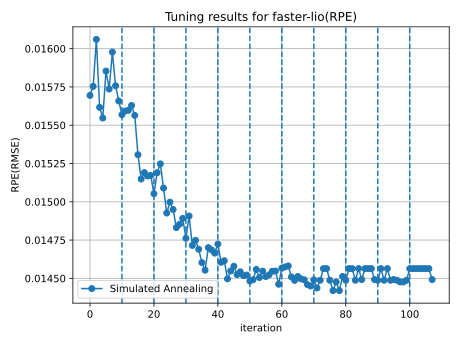
\includegraphics[width=0.65\linewidth]{images/faster-lio-sa.pdf}
    \caption{RPE per iteration of Simulated Annealing}
    \label{faster-lio-sa}
\end{figure}

%\paragraph{}The vertical dotted lines represent the iterations where the temperature was reset to its initial value(reannealing). 

\paragraph{}From Figure \ref{faster-lio-sa}, it can be seen that, roughly for the first 80 iterations, reannealing (vertical dotted lines) allows the algorithm to escape local minima and achieve a better solution than the incumbent. After this point, the algorithm stagnated, with no further improvements observed for nearly 30 iterations, which was therefore selected as the stopping criterion. While this parameter is configurable, preliminary experiments conducted on a 30-second segment of the dataset suggested limited benefit in extending the optimization beyond this threshold. Additionally, due to the considerable runtime of each simulated annealing run (approximately 2.5 minutes per iteration, amounting to 2–5 hours for 50–100 iterations), certain pragmatic compromises were required. The most important one was that most optimizations, in terms of parameter settings, such as delta\_max for discrete parameters or gaussian curve $\mu$ and $\sigma$ values for continuous parameters were adjusted while working with 30 second sections of the dataset. While it does not guarantee that such adjustments will work on the entire dataset, it allows the researcher to understand how their values affect algorithm runtime and performance.


%After that, it gets stuck and doesn't go anywhere for almost 30 iterations, which was the limit proposed for halting the execution, when no better solution is found. This parameter is customizable, but it was decided, after a few runs with a 30 second section of the dataset, that it was not productive to let the algorithm run for so long without achieving any better solution. Also, given the time each Simulated Annealing run takes(2.5 minutes x ([50, 100] iterations) = [2, 5] hours), some shortcuts had to be taken. The most important one was that most optimizations, in terms of parameter settings, such as delta\_max for discrete parameters or gaussian curve $\mu$ and $\sigma$ values for continuous parameters were adjusted while working with 30 second sections of the dataset. While it does not guarantee that such adjustments will work on the entire dataset, it allows the researcher to understand how their values affect algorithm runtime and performance.

\begin{figure}[h]
    \centering
    \includegraphics[width=0.75\linewidth]{images/cube_side_length_rpe.pdf}
    \caption{cube\_side\_length scatter plot}
    \label{cube_side_length_scatter}
\end{figure}

\paragraph{}Figure \ref{cube_side_length_scatter} shows the scatter plot for the discrete parameter cube\_side\_length. It indicates the optimal range for this parameter is between 1300 and 1700. This is not conclusive, however. Correlation does not mean causation. Other parameters were tuned and their effects on the \ac{RPE} may be greater, such as ivox\_grid\_resolution (Figure \ref{ivox_grid_resolution_scatter}). In this case, the relationship between parameter value and the \ac{RPE} is even clearer, for there seems to be an almost linear relationship between parameter value and \ac{RPE}. %Although filter\_size\_surf seems to stabilize for values between 0.25 and 0.5, it was decided to explore even lower values. For ivox\_grid\_resolution, the lower bound was defined as 0.1, hence why there weren't any values below it. Even though there the scatter plot shows a possible linear relationship between this parameter and the \ac{RPE}, it might be worthwhile to explore lower ivox\_grid\_resolution values. For the parameters filter\_size\_map and esti\_plane\_threshold, the scatter plots looked very similar to filter\_size\_surf and ivox\_grid\_resolution, and a similar reasoning regarding further optimization was applied.

\begin{figure}[h]
    \centering
    \includegraphics[width=0.65\linewidth]{images/ivox_grid_resolution_rpe.pdf}
    \caption{ivox\_grid\_resolution scatter plot}
    \label{ivox_grid_resolution_scatter}
\end{figure}

\paragraph{}These scatter plots serve as a visual aid to the researcher to better analyze and understand the relationships between tuned parameter values and target metric values.

\subsection{Grid Search}

\paragraph{}Grid Search was run for 5 hours. Its \ac{RPE} per iterations is shown in Figure \ref{faster-lio-grid-search-rpe}.

\begin{figure}[h]
    \centering
    \includegraphics[width=0.6\linewidth]{images/faster-lio-gs.pdf}
    \caption{RPE per iterations of Grid Search}
    \label{faster-lio-grid-search-rpe}
\end{figure}

%\paragraph{}As with Simulated Annealing, a few scatter plots are necessary to try to make sense of these results. Below are the three scatter plots which are necessary to understand these results(figures \ref{faster-lio-grid-search-filter_size_map}, \ref{faster-lio-grid-search-filter_size_surf} and \ref{faster-lio-grid-search-ivox_grid_resolution}).

\paragraph{}As with Simulated Annealing, several scatter plots are required to facilitate the interpretation of these results. Figures \ref{faster-lio-grid-search-filter_size_map}, \ref{faster-lio-grid-search-filter_size_surf} and \ref{faster-lio-grid-search-ivox_grid_resolution} present such scatter plots.

\begin{figure}[h]
    \centering
    \includegraphics[width=0.6\linewidth]{images/fasterliogs-ivox-grid-resolution.pdf}
    \caption{ivox\_grid\_resolution scatter plot}
    \label{faster-lio-grid-search-ivox_grid_resolution}
\end{figure}

\begin{figure}[h]
    \centering
    \includegraphics[width=0.6\linewidth]{images/fasterliogs-filter-size-map.pdf}
    \caption{filter\_size\_map scatter plot}
    \label{faster-lio-grid-search-filter_size_map}
\end{figure}

\begin{figure}[h]
    \centering
    \includegraphics[width=0.6\linewidth]{images/fasterliogs-filter-size-surf.pdf}
    \caption{filter\_size\_surf scatter plot}
    \label{faster-lio-grid-search-filter_size_surf}
\end{figure}

\paragraph{}The first thing to note is that all tuned parameters have a pattern equal to that of ivox\_grid\_resolution, hence they are not relevant. The reason for this pattern is the sequential nature of Grid Search.

\paragraph{}Secondly, the filter\_size\_map parameter does not seem to affect the \ac{RPE} at all, given how sparsely distributed the scatter plot points are. However,  filter\_size\_surf seems to be the only tuned parameter that significantly affects the \ac{RPE}, having an almost linear relationship. However, given the Simulated Annealing results discussed previously, and specifically figures \ref{ivox_grid_resolution_scatter} and \ref{cube_side_length_scatter}, it can be argued that the apparent lack of influence of parameters such as ivox\_grid\_resolution and cube\_side\_length on the overall \ac{RPE} is a consequence of the limited coverage of the parameter space achieved by the Grid Search algorithm. At best, the results indicate that, when all parameters except filter\_size\_map and filter\_size\_surf are held fixed, the observed performance is obtained locally. However, this provides limited insight into the globally optimal parameter configuration for sequence 1006\_03 of the BotanicGarden dataset.

%it is possible to assert that the reason parameters such as ivox\_grid\_resolution and cube\_side\_length \textbf{look} like they have no effect on the overall \ac{RPE} value is that Grid Search did not do a comprehensive enough search of the parameter space. At most it can be concluded that \textbf{locally}, fixating the values of all parameters except for filter\_size\_map and filter\_size\_surf, these results are achieved. But that does not tell us much about the global optimal parameters(for sequence 1006\_03 of the BotanicGarden dataset).

%\paragraph{}The first thing that comes to mind by looking at figure \ref{faster-lio-grid-search-rpe} is how high the \ac{RPE} values are. This is because of a few reasons.

%\paragraph{}Firstly, only 1\% of the parameter space(total of 11000 configurations) was explored. Exploring such a tiny fraction of the parameter space does not yield conclusive results about the optimal parameter values. However, in these circumstances, we do not start from default parameters and attempt to find the most optimal values for all parameters. In theses circumstances, we started with the results of a previous optimization algorithm(Simulated Annealing), and devised a much narrower parameter space considering previous results and potential areas of improvement, to try to further improve the \ac{RPE}. Even though the expectations for further \ac{RPE} improvements were low, it cannot be concluded that the \ac{RPE} has reached its lowest value.

%S\paragraph{}Secondly, the parameter space is very small, even though only 4 out of the 7 initial parameters are being optimized here, and each parameter can only take 10/11 possible values. The step size values for each parameter determine how fined grained the search is. A very low step size could mean large regions of the parameter space have identical \ac{RPE} values, and the search in those regions wouldn't be productive.

%\paragraph{}Given all that, it was decided to run Random Search on the same parameter space, and only then decide, based on its results, if the parameter space should be larger(bigger step sizes + total number of values) or if the results can be considered "as is".

\subsection{Random Search}

\paragraph{}For Random Search, the same parameter space was used, and the algorithm was run for 5 hours, as was the case with Grid Search. In total, both algorithms were run for a total of 100 iterations. Figure \ref{faster-lio-random-search-rpe} illustrates the \ac{RPE} per iteration of Random Search.

%Below is a figure of the \ac{RPE} per iteration of Random Search(figure).

\begin{figure}[h]
    \centering
    \includegraphics[width=0.65\linewidth]{images/faster-lio-rs.pdf}
    \caption{RPE per iterations of Random Search}
    \label{faster-lio-random-search-rpe}
\end{figure}

\newpage

%\paragraph{}One of the first things that comes to mind when looking at figure \ref{faster-lio-random-search-rpe} are the outliers and how it distorts the plot and makes it very difficult to know the y-axis value of most points. The reason is very simple: Random Search is randomly sampling a configuration out of the 11000 possible configurations, and some of those configurations have much larger \ac{RPE} values.

%\paragraph{}The best performing configuration achieved an \ac{RPE} of 0.014405. To put that into perspective, Simulated Annealing achieved 0.014420. This comparison is not obviously fair, given that the parameter space that was used in Random Search was designed \textbf{after} analyzing the results of Simulated Annealing. Also, the difference between the two best performing configurations is not significant enough to conclude anything about the the best performing region in the parameter space.

%\paragraph{}Random Search was mainly used to demonstrate its advantages. One, It outperforms Grid Search in time constrained environments, finding better performing regions of the parameter space randomly. Secondly, in general, it might be a good tool to randomly sample the parameter space for promising regions before moving on to more advanced approaches using more efficient tuning algorithms, provided time constraints are not as "tight" and the parameter space is highly granular, meaning the step sizes are very low, and each parameter is given thousands(possibly millions, depending on the machine's hardware) of possible values.

\paragraph{}For the scatter plots, the two outlier points were removed, to undo the scale distortion. As with Grid Search, the scatter plots for ivox\_grid\_resolution (Figure \ref{faster-lio-random-search-ivox_grid_resolution}), filter\_size\_map (Figure \ref{faster-lio-random-search-filter_size_map}) and filter\_size\_surf (Figure \ref{faster-lio-random-search-filter_size_surf}) are presented.

\begin{figure}[h]
    \centering
    \includegraphics[width=0.6\linewidth]{images/fasterliors-ivox-grid-resolution.pdf}
    \caption{ivox\_grid\_resolution scatter plot}
    \label{faster-lio-random-search-ivox_grid_resolution}
\end{figure}

\begin{figure}[h]
    \centering
    \includegraphics[width=0.6\linewidth]{images/fasterliors-filter-size-map.pdf}
    \caption{filter\_size\_map scatter plot}
    \label{faster-lio-random-search-filter_size_map}
\end{figure}

\begin{figure}[h]
    \centering
    \includegraphics[width=0.6\linewidth]{images/fasterliors-filter-size-surf.pdf}
    \caption{filter\_size\_surf scatter plot}
    \label{faster-lio-random-search-filter_size_surf}
\end{figure}

%\paragraph{}The previous three figures allow us to get a better picture of how these parameters influence the \ac{RPE} value. In all three cases, all 9 possible values are explored, showcasing the main advantage of Random Search over Grid Search: with a fixed optimization constraint(in this case, a time limit of 5 hours) and a large enough parameter space(157464 configurations), Random Search not only explores the parameter space better, but also tends to achieve better results.

\newpage
\paragraph{}The previous three figures provide a clearer understanding of how these parameters affect the \ac{RPE}. In each case, all nine possible values are examined, highlighting the primary advantage of Random Search over Grid Search: given a fixed optimization constraint (in this case, a time limit of five hours) and a sufficiently large parameter space (157464 configurations), Random Search not only explores the space more effectively but also generally achieves superior results.

\paragraph{}Table \ref{faster-lio table} sums up the results of the tuning process for Faster-LIO.

\begin{table}[h]
\centering
\begin{tabular}{c|c|c|}
\cline{2-3}
\multicolumn{1}{l|}{}                       & RPE      & \% difference to default configuration \\ \hline
\multicolumn{1}{|c|}{Default configuration} & 0.015037 & +0\%  \\ \hline
\multicolumn{1}{|c|}{Grid Search}           & 0.015297 & +1.73\% \\ \hline
\multicolumn{1}{|c|}{Random Search}         & 0.015298 & +1.74\% \\ \hline
\multicolumn{1}{|c|}{Simulated Annealing}   & 0.014420 & -4.1\%  \\ \hline
\end{tabular}
\caption{Faster-LIO tuning results}
\label{faster-lio table}
\end{table}

\section{Fast-LIVO2}

\paragraph{}As was the case with Faster-LIO, prior to parameter tuning, Fast-LIVO2 was evaluated using its default parameter configuration to establish a baseline for \ac{RPE}. Table \ref{default-fast-livo2} presents the five-run average APE and RPE for Fast-LIVO2, obtained using the parameter values reported in Table \ref{default-fast-livo2-params}.

\begin{table}[h]
\centering
\begin{tabular}{|l|l|}
\hline
APE (RMSE) & RPE (RMSE) \\ \hline
0.403815  & 0.045583  \\ \hline
\end{tabular}
\caption{Default parameter results (5 run average) for Fast-LIVO2}
\label{default-fast-livo2}
\end{table}

\newpage

\begin{table}[h]
\centering
\begin{tabular}{|l|l|}
\hline
point\_filter\_num     & 1    \\ \hline
max\_iterations        & 5    \\ \hline
filter\_size\_pcd      & 0.15 \\ \hline
filter\_size\_surf     & 0.1  \\ \hline
half\_map\_size        & 100  \\ \hline
patch\_pyrimid\_level  & 4    \\ \hline
max\_points\_num       & 50   \\ \hline
patch\_size            & 8    \\ \hline
max\_layer             & 2    \\ \hline
outlier\_threshold     & 1000 \\ \hline
sliding\_thresh        & 8    \\ \hline
voxel\_size            & 0.5  \\ \hline
\end{tabular}
\caption{Default parameter values for Fast-LIVO2}
\label{default-fast-livo2-params}
\end{table}

\paragraph{}Before running Simulated Annealing, it is necessary to define the hyperparameters of the tuning algorithm.

\paragraph{}Then, the following parameter space was devised. The two tables below present the parameter settings used for Simulated Annealing. The parameters are divided into two groups: discrete parameters (Table \ref{fast-livo2-discrete-params-settings}) and continuous parameters (Table \ref{fast-livo2-continuous-params-settings}).

\begin{table}[h]
\centering
\begin{tabular}{|c|c|c|c|c|}
\hline
Parameter             & Initial Value & Lower Bound & Upper Bound & delta max \\ \hline
point\_filter\_num    & 100           & 5           & 150         & 20        \\ \hline
max\_iterations       & 70            & 40          & 95          & 15        \\ \hline
patch\_size           & 18            & 5           & 25          & 10        \\ \hline
patch\_pyrimid\_level & 18            & 4           & 32          & 7         \\ \hline
max\_layer            & 25            & 2           & 50          & 10        \\ \hline
max\_points\_num      & 105           & 90          & 120         & 50        \\ \hline
half\_map\_size       & 400           & 75          & 750         & 150       \\ \hline
sliding\_thresh       & 15            & 8           & 25          & 7         \\ \hline
outlier\_threshold    & 4000          & 750         & 7500        & 1500      \\ \hline
\end{tabular}
\caption{Fast-LIVO2 discrete parameter settings}
\label{fast-livo2-discrete-params-settings}
\end{table}

\newpage
\begin{table}[h]
\centering
\begin{tabular}{|c|c|c|c|c|c|}
\hline
Parameter          & Initial Value & Lower Bound & Upper Bound & $\mu$  & $\sigma$ \\ \hline
filter\_size\_surf & 1.45          & 0.1         & 5.0         & -0.035 & 0.003    \\ \hline
voxel\_size        & 2.5           & 0.2         & 17.75       & -0.055 & 0.003    \\ \hline
\end{tabular}
\caption{Fast-LIVO2 continuous parameter settings}
\label{fast-livo2-continuous-params-settings}
\end{table}

\begin{figure}[h]
    \centering
    \includegraphics[width=0.65\linewidth]{images/fast-livo2-sa.pdf}
    \caption{RPE per iteration of Simulated Annealing}
    \label{fast-livo2-sa}
\end{figure}

\paragraph{}From Figure \ref{fast-livo2-sa}, it can be seen that, roughly for the first 70 iterations, reannealing allows the algorithm to escape local minima and achieve a better solution than the incumbent. After this point, the algorithm seemed to stagnate, with no further improvements observed until iteration 100, after which it halted its execution. Due to the considerable runtime of each simulated annealing run (approximately 2.5 minutes per iteration, amounting to 2–5 hours for 50–100 iterations), as well as the increased number of parameters of Fast-LIVO2 relative to Faster-LIO, some conclusions can be drawn. One, Simulated Annealing requires constant interaction and feedback from the tuner in order to adjust the algorithm hyperparameters, particularly the perturbation functions' settings, taking several runs before performance reaches acceptable levels.

\newpage
\begin{figure}[h]
    \centering
    \includegraphics[width=0.65\linewidth]{images/fast-livo2-sa-filter_size_pcd.pdf}
    \caption{filter\_size\_pcd scatter plot}
    \label{fast-livo2-filter_size_pcd_scatter}
\end{figure}

\paragraph{}Figure \ref{fast-livo2-filter_size_pcd_scatter} shows the scatter plot for the continuous parameter filter\_size\_pcd. It seems to indicate the optimal range for this parameter is between 0.2 and 0.75. This is not conclusive, however, as other tuned parameters' scatter plots displayed a similar pattern (see figure \ref{fast-livo2-point_filter_num_scatter}), indicating multiple parameters with a strong quasi-linear relationship with the \ac{RPE}.

\begin{figure}[h]
    \centering
    \includegraphics[width=0.6\linewidth]{images/fast-livo2-sa-point_filter_num.pdf}
    \caption{point\_filter\_num scatter plot}
    \label{fast-livo2-point_filter_num_scatter}
\end{figure}

\subsection{Grid Search}

\paragraph{}Similarly to Faster-LIO, Grid Search was run Fast-LIVO2 for 5 hours. Its \ac{RPE} per iterations is shown in Figure \ref{fast-livo2-grid_search}.

\begin{figure}[h]
    \centering
    \includegraphics[width=0.7\linewidth]{images/fast-livo2-gs.pdf}
    \caption{RPE per iteration for Grid Search}
    \label{fast-livo2-grid_search}
\end{figure}

\paragraph{}As with Simulated Annealing, several scatter plots are required to facilitate the interpretation of these results. Figures \ref{fast-livo2-grid_search-filter_size_pcd} and \ref{fast-livo2-grid_search-outlier_threshold} present such scatter plots.

\begin{figure}[h]
    \centering
    \includegraphics[width=0.6\linewidth]{images/fast-livo2-gs-filter_size_pcd_rpe.pdf}
    \caption{filter\_size\_pcd scatter plot}
    \label{fast-livo2-grid_search-filter_size_pcd}
\end{figure}

\begin{figure}[h]
    \centering
    \includegraphics[width=0.6\linewidth]{images/fast-livo2-gs-outlier_threshold_rpe.pdf}
    \caption{outlier\_threshold scatter plot}
    \label{fast-livo2-grid_search-outlier_threshold}
\end{figure}

\newpage
\paragraph{}The first thing that should be noted is that while in Faster-LIO seven parameters were tuned, in Fast-LIVO2 there are twelve parameters being tuned, and therefore, taking into account practical limitations, this means the parameter space is necessarily sparser and not detailed enough for a conclusive analysis. Despite that, Grid Search still manages to achieve an \ac{RPE} value of 0.0316, which is about 30.5\% lower than the default configuration.

\subsection{Random Search}

\paragraph{}As before, for Random Search, the same parameter space was used, and the algorithm was run for 5 hours, as was the case with Faster-LIO. In total, both algorithms were run for a total of 100 iterations. Figure \ref{faster-lio-random-search-rpe} illustrates the \ac{RPE} per iteration of Random Search.

%Below is a figure of the \ac{RPE} per iteration of Random Search(figure).

\begin{figure}[h]
    \centering
    \includegraphics[width=0.6\linewidth]{images/fast-livo2-rs.pdf}
    \caption{RPE per iterations of Random Search}
    \label{fast-livo2-rs}
\end{figure}

\paragraph{}As with Grid Search, the scatter plots for filter\_size\_pcd (Figure \ref{fast-livo2-random_search-filter_size_pcd}) and outlier\_threshold (Figure \ref{fast-livo2-random_search-outlier_threshold}) are presented.


\begin{figure}[h]
    \centering
    \includegraphics[width=0.6\linewidth]{images/fast-livo2-rs-filter_size_pcd_rpe.pdf}
    \caption{filter\_size\_pcd scatter plot}
    \label{fast-livo2-random_search-filter_size_pcd}
\end{figure}

\begin{figure}[h]
    \centering
    \includegraphics[width=0.6\linewidth]{images/fast-livo2-rs-outlier_threshold_rpe.pdf}
    \caption{outlier\_threshold scatter plot}
    \label{fast-livo2-random_search-outlier_threshold}
\end{figure}

\paragraph{}Unlike Faster-LIO, it is not possible to derive any meaningful conclusions from the Random Search scatter plots for Fast-LIVO2. Even though Random Search managed to achieve an \ac{RPE} value 5.4\% lower than Grid Search, mostly due to its pseudo-random nature, the increased number of tuned parameters for Fast-LIVO2, as mentioned previously, forces the tuner to design a low resolution search space, limiting the potential benefits.

\newpage
\paragraph{}Table \ref{fast-livo2-table} sums up the results of the tuning process for Fast-LIVO2.

\begin{table}[h]
\centering
\begin{tabular}{c|c|c|}
\cline{2-3}
\multicolumn{1}{l|}{}                       & RPE      & \% difference to default configuration \\ \hline
\multicolumn{1}{|c|}{Default configuration} & 0.045583 & +0\%                                   \\ \hline
\multicolumn{1}{|c|}{Grid Search}           & 0.031670 & -30.52\%                               \\ \hline
\multicolumn{1}{|c|}{Random Search}         & 0.029969 & -34.25\%                               \\ \hline
\multicolumn{1}{|c|}{Simulated Annealing}   & 0.006979 & -84.69\%                               \\ \hline
\end{tabular}
\caption{Fast-LIVO2 tuning results}
\label{fast-livo2-table}
\end{table}





